\documentclass[12pt, a4paper]{article}

\usepackage{geometry}
\usepackage{graphicx}
\graphicspath{./}
\geometry{
  a4paper,
  total={170mm,257mm},
  left=20mm,
  top=20mm,
}
\usepackage{hyperref}
\hypersetup{
  colorlinks=true,
  linkcolor=blue,
  filecolor=magenta,      
  urlcolor=cyan,
  pdftitle={Overleaf Example},
  pdfpagemode=FullScreen,
}

\title{Build Your PC}
\author{Zakariyya Kurmally (Student ID: 2315839)}

\begin{document}
\maketitle
\pagebreak
\tableofcontents
\pagebreak

% Requirements %

\section{Requirements}

\subsection{Programming}
The final build should be able to excecute build tasks at a decent speed
so processor, memory and SSD choices should take this into account.

\subsection{Quiet}
The PC should be as quiet as possible. As such, parts that require 
massive amounts of cooling are out of the question. This will also
affect fan choice.

\subsection{Open Source Drivers}
Since the computer will be running GNU/Linux, it will be preferable if most of 
the parts have drivers which are open-source. This means no Nvidia.

\subsection{Budget}
Ideally, the parts should offer a decent performance whilst being
relatively affordable. The budget for this build shall be around
\$500.

% End Requirements %

% Parts Investigation %

\section{Parts Investigation}
% This section shall cover different parts considered and will focus on the 
% following aspects:
% \begin{itemize}
%   \item Cost 
%   \item Availability 
%   \item Performance
% \end{itemize}

\subsection{Processor}
\begin{center}
  % Techspot - Anatomy of a CPU
  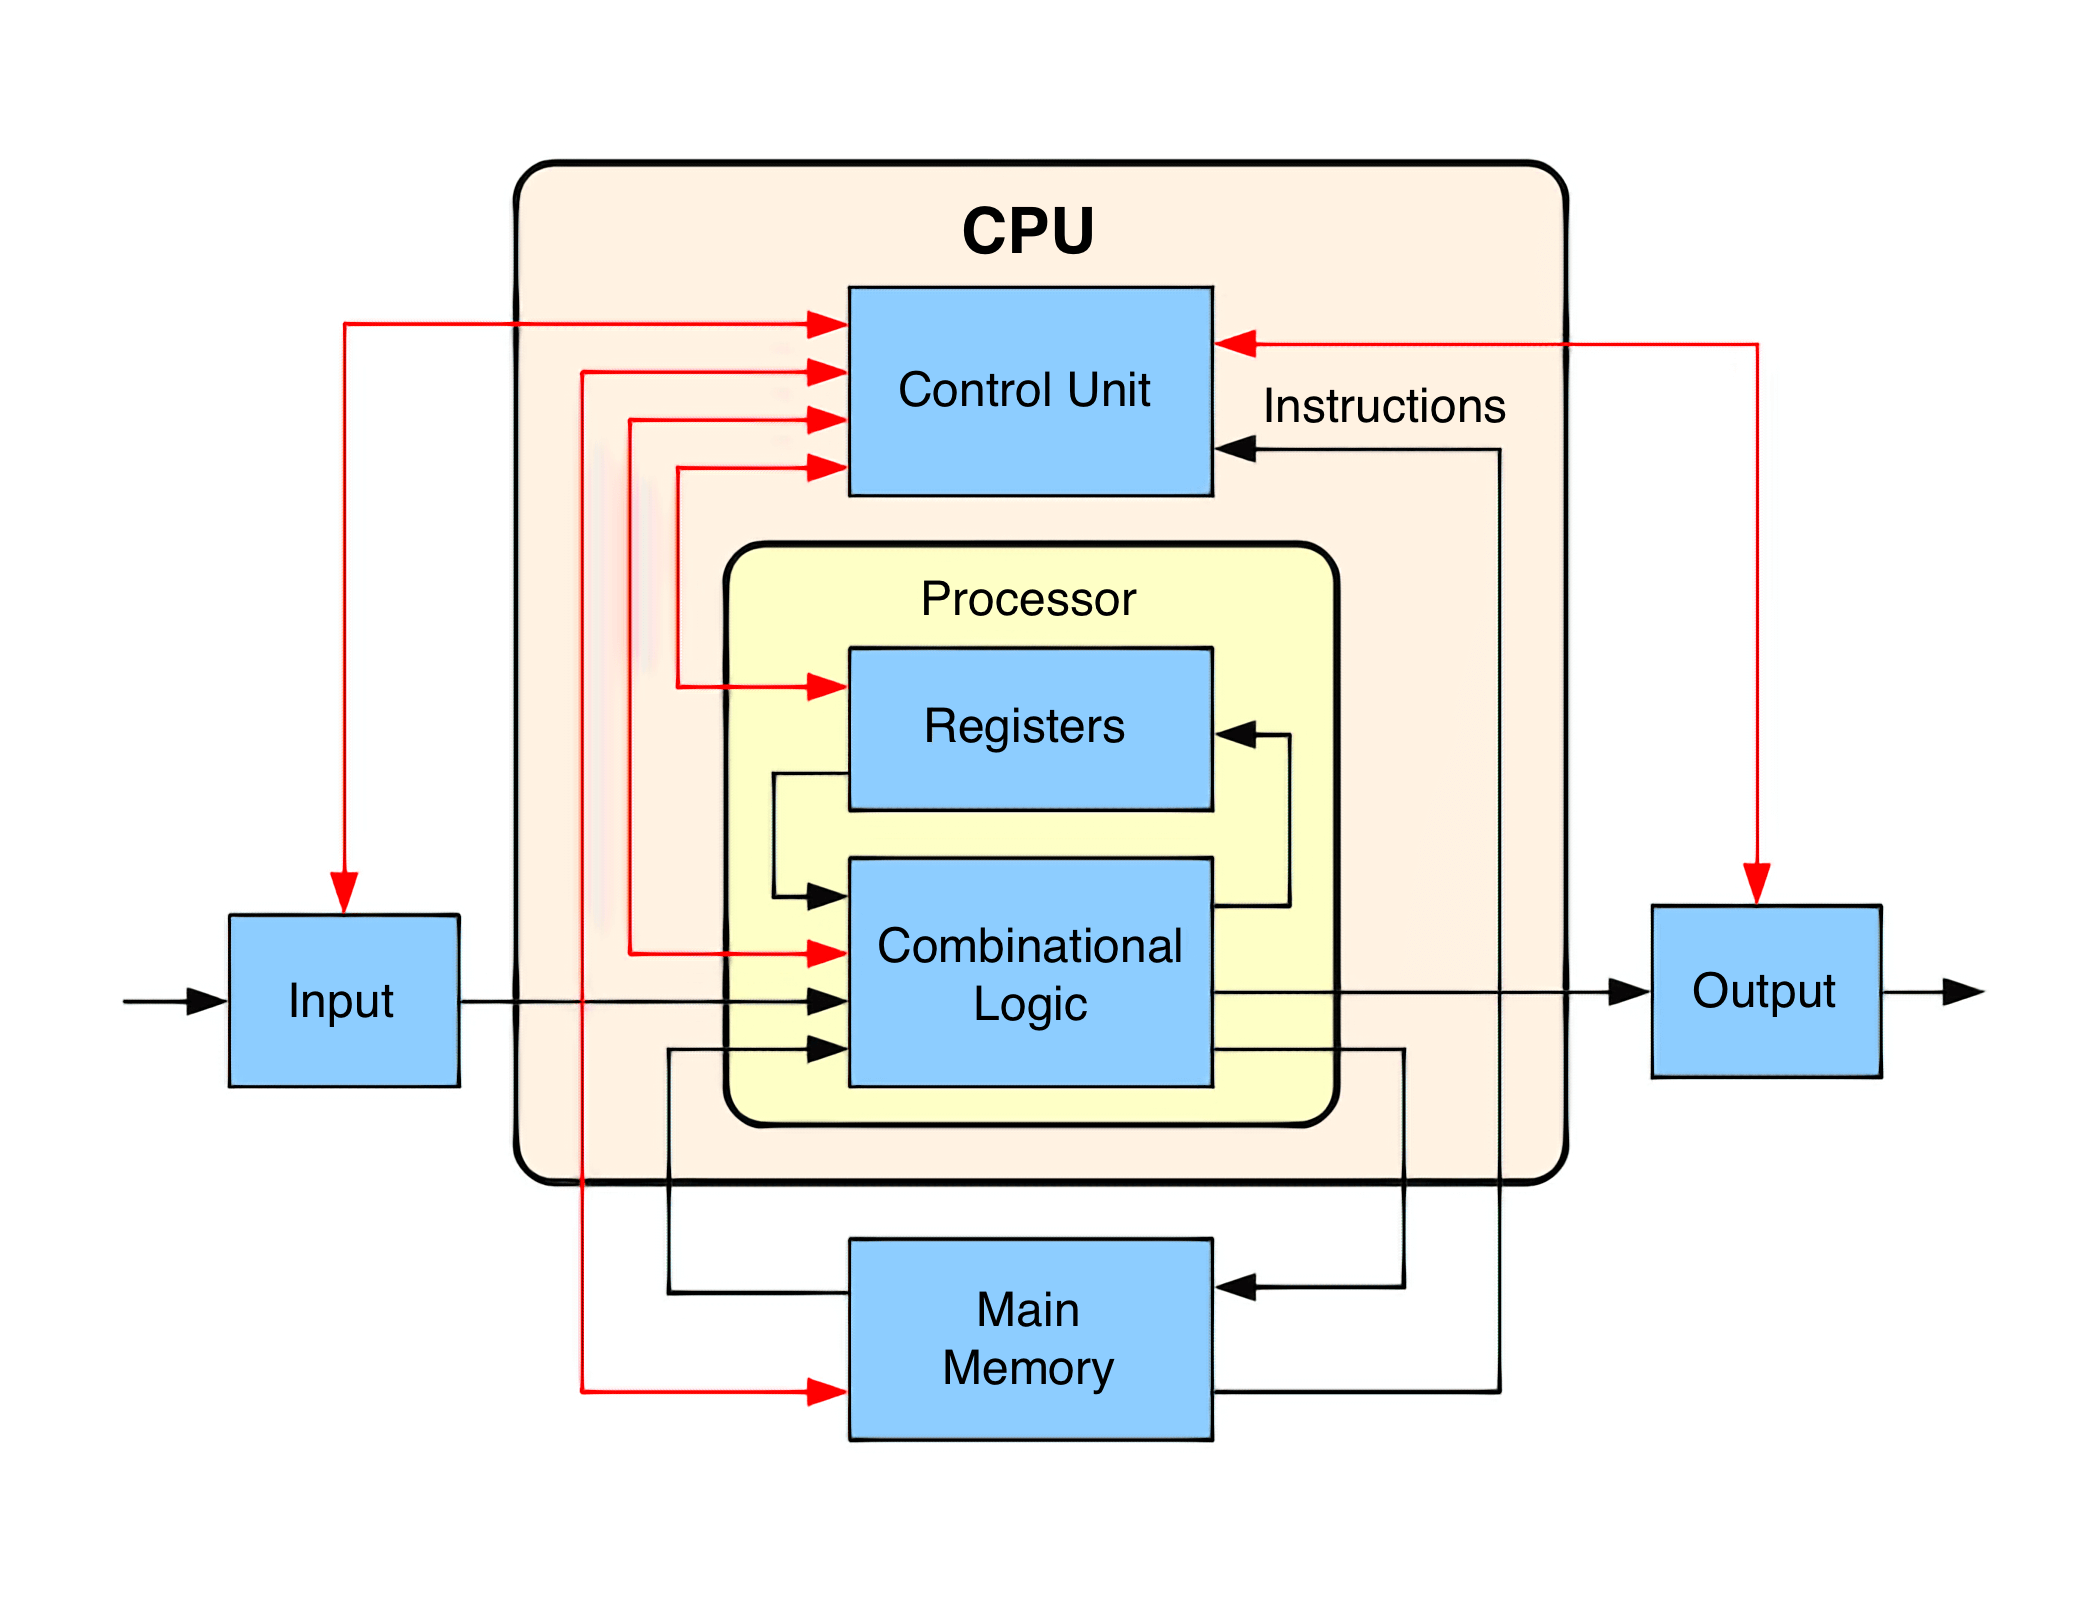
\includegraphics[scale=0.15]{cpu.png}
\end{center}

The above is an image showing the basic internals of a CPU. A CPU can be 
considered to be the primary component of a computer. It is often 
referred to as the "brain" of the computer since it is responsible
for arithmetic, logic, control and input/output operations specified by 
instructions in the computer's program. 

The two main competitors in this space are AMD and Intel. Over the years,
both have whipped out decent budget alternatives. This section will look
at what both sides can offer with respect to the aforementioned 
requirements.

\subsection{Motherboard}
\begin{center}
  % Techspot - Motherboard
  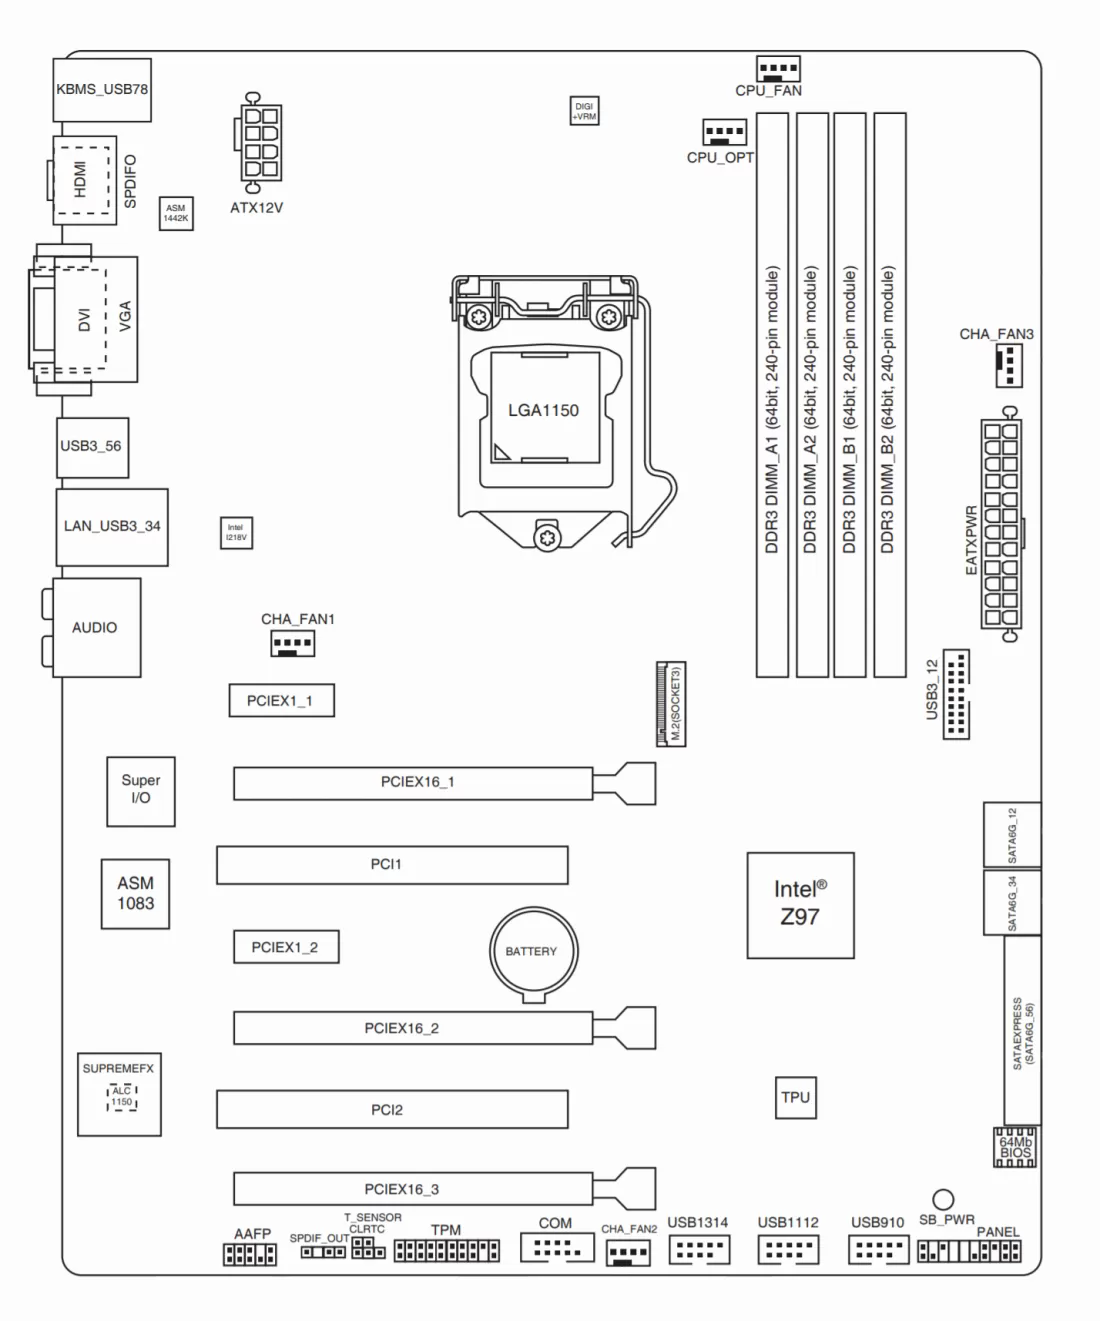
\includegraphics[scale=0.2]{motherboard.png}
\end{center}

A motherboard is the main printed circuit board (PCB) in a computer.
It serves as the foundation upon which other parts are built upon. 
It connects all the parts of the machine together. It consist of many 
parts as shown on the diagram above.

\subsection{RAM}
Random Access Memory is a form of volatile memory in a computer system
responsible for the temporary storage of data and instructions currently
being executed.

\subsection{Storage}
These include storage devices that are not directly accessible by the CPU.
They are non-volatile devices which allow data to be stored for as long
as the user needs. In terms of capacity, they are much larger than main
memory but access times are slower. Applications, the operating system,
device drivers and general files are stored in secondary storage. This
system will consider the following 2 types of secondary storage:
\begin{itemize}
  \item Hard Disk Drives: Makes use of magnetic storage technology with 
    moving parts. HDDs have slower access and data transfer speeds. They
    are also less durable and make more noise since they have 
    moving parts but are generally more affordable. 
  \item Solid State Drives: Uses flash technology and stores data in 
    non-volatile memory chips (usually NAND). They do not make use
    of moving parts and are hence quieter, smaller and more durable. 
    However they tend to be more expensive.
\end{itemize}

\subsection{Power Supply Unit}
As its name suggests, a Power Supply Unit (PSU) provides power to the 
system. In more precise terms, it converts electrical power from an outlet
to the appropriate direct current voltages required by the computer parts.
Some of its key responsibilities are: voltage regulations, provision
of connectors, modularity and safety features.

\subsection{Case}
A case provides an enclosure where other parts of the computer live in.
They come in different shapes and sizes to accommodate for different
configurations a user a opt for when building a PC. Cases serve the 
following purposes, amongst others:
\begin{itemize}
  \item Protection: protects the internal components from dust, moisture
    and other factors that could damage the internals.
  \item Cooling: many cases are designed with airflow and cooling in mind.
    With strategically placed vents and cable management systems, some cases
    allow for optimal airflow leading to optimal performance of hardware and
    prevention of thermal throttling.
\end{itemize}

% End Parts Investigation %

% Parts Selection %

\section{Parts Selection}
This section will concern itself with parts from Amazon. Any price
and brands mentioned have been taken at the time of writing from
Amazon.

\begin{center}
  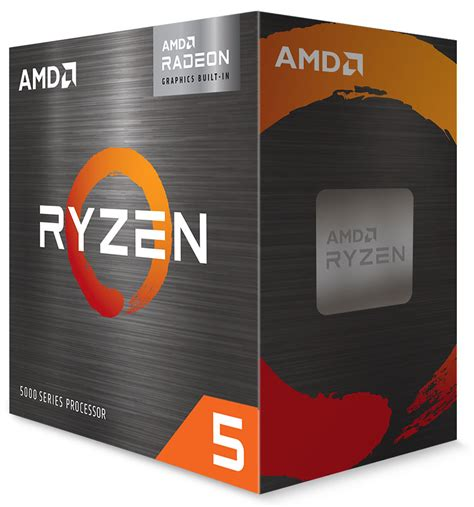
\includegraphics[scale=0.2]{ryzen.png}
\end{center}

Sitting around \$125, the ryzen 5 5600G offers 6 cores, clocked at 3.5 GHz
base, and 12 threads, this processor offers a great balance between price
and performance. It is also widely available on Amazon and Ebay. 
Furthermore, it comes with pre-applied thermal paste and a cooler. Finally,
the integrated graphics module will be more than enough for desktop use
and will save on noise which a dedicated GPU would have produced.

\vspace{4pt}
\begin{center}
  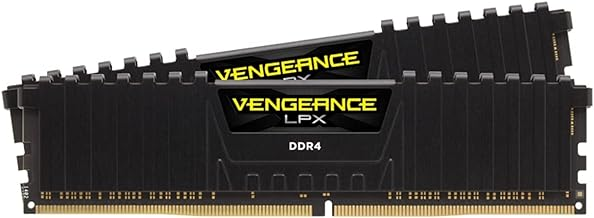
\includegraphics[scale=0.29]{el_ram_de_comer.jpg}
\end{center}

To complement our processor, the Corsair Vengeance LPX DDR4 will fit our
needs for \$45. It consists of 2 sticks of 8GB, clocked at 3200 MHz
with XMP available.

\vspace{4pt}
\begin{center}
  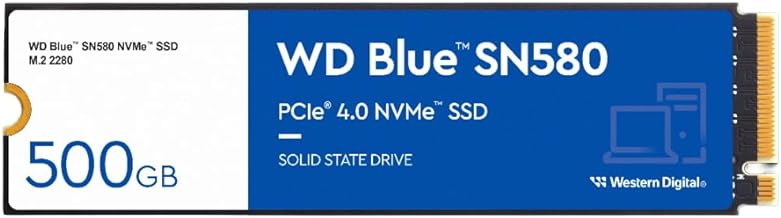
\includegraphics[scale=0.2]{ssssssssssssd.jpg}
\end{center}

The Western Digital NVMe SSD offers Gen 4 PCIe speeds at \$57.

\vspace{4pt}
\begin{center}
  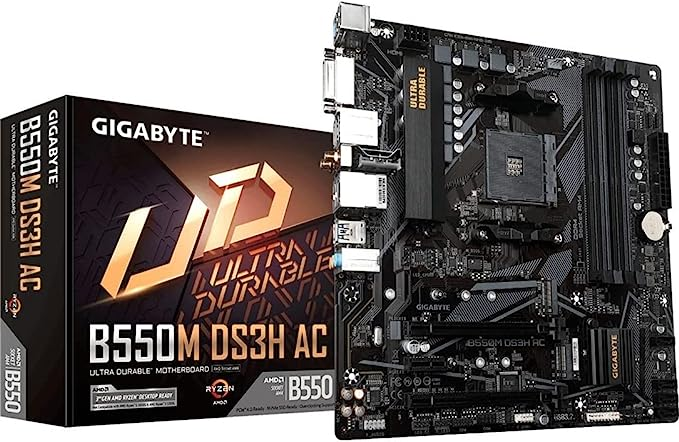
\includegraphics[scale=0.32]{mothaaaaaaaaaaa.jpg}
\end{center}

The Gigabyte B550M DS3H AC will be able to house the aforementioned
parts comfortably. It has built-in Wifi and supports dual-channel 
memory. At \$99, this will be a bargain.

\vspace{4pt}
\begin{center}
  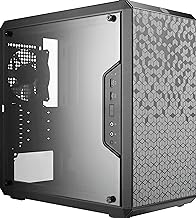
\includegraphics[scale=0.6]{colaaaaaaaaaa.jpg}
\end{center}

The Cooler Master MasterBox Q300L Micro-ATX Tower comes with an included
fan and will be able to house our parts for \$40. 

\vspace{4pt}
\begin{center}
  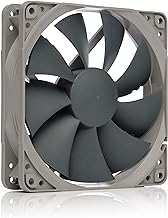
\includegraphics[scale=0.6]{faaaaaaannnnn.jpg}
\end{center}
The Noctua NF-P12 will be used as a front intake fan. Noctua is known
for its silent fans. This will set us back \$15.

\vspace{4pt}
\begin{center}
  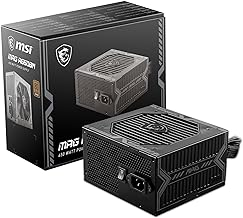
\includegraphics[scale=0.6]{can_you_feel_the_powaaaaaaaa.jpg}
\end{center}
With its 650 watts, the MSI MAG A650BN will be more than enough to
power our whole system for \$60.

% End Parts Selection %

% Motherboard Labelling %

\section{Motherboard Labelling}
Provided by \href{https://www.gigabyte.com/Motherboard/B550M-DS3H-rev-10-11-12-13\#kf}{Gigabyte}:
\vspace{4pt}
\begin{center}
  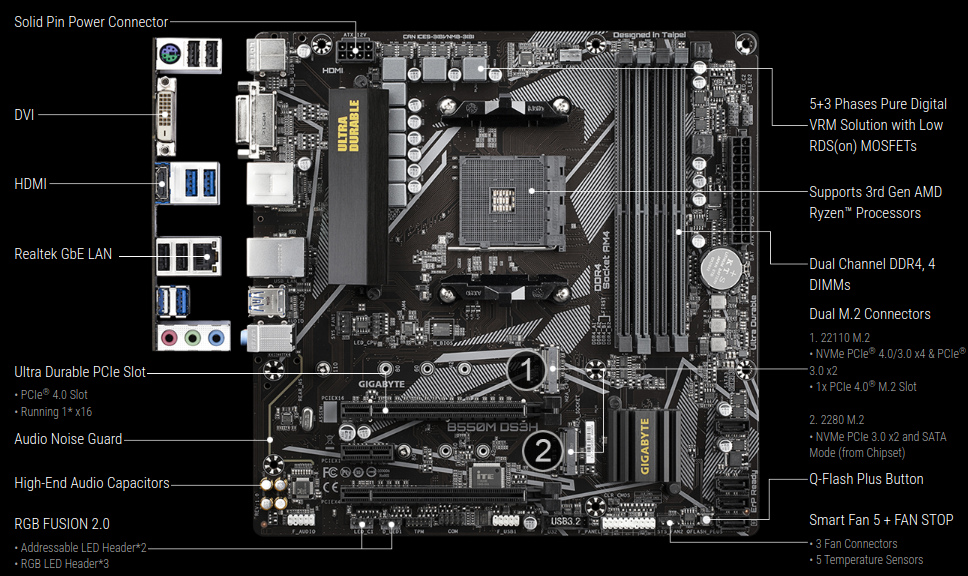
\includegraphics[scale=0.6]{unga.png}
\end{center}

% EndMotherboard Labelling %

% Operating System %

\section{Operating System}
Linux. No debate. MacOS is only supported on devices Apple sells; legally
anyways. And windows is a nightmare on its own. The sheer amount of resources
it takes while idle is mind boggling. Windows also dominates in the market
share for viruses with over 83\% of all viruses in 2020 designed for it.
Furthermore, windows is an operating system that just gets in the way.
Need to find a package or library? Spend an ungodly amount of time
scouring websites to find it and hope it does not contain any malware.
Moreover, in terms of personal configurations, it's like scraping the 
bottom of the barrel. Hence, Linux, more precisely Arch shall be my OS of
choice for this PC. Here are a couple more advantages:

\begin{itemize}
  \item Pacman: It is the package manager for Arch Linux. Any package can 
    be installed with 'sudo pacman -S <package name>'. It also supports 
    parallel downloading. In addition, Pacman has many frontends such 
    as Yay which can easily download and install packages which are
    not in the main repositories.
  \item Customisability: Linux is extremely modular by nature. Almost
    anything from the desktop environment to the kernel itself can
    be modified to fit the user's need. With Linux, the computer changes
    itself to accommodate the user, not the other way around.
  \item Privacy: Being open-source means that Linux is very transparent
    by nature. As such, no hidden data collection or spyware running in 
    the background.
  \item Programming environment: with support for many languages available
    by default and others just a command away, Linux is considered
    by some to be the ideal coding environment. Furthermore, any libraries
    or dependencies are simpler to deal with on Posix systems as most 
    of them are available via the package managers.
\end{itemize}

% End Operating System %

\section{Conclusion}
All in all, the build fits the requirements. All the parts have drivers
widely supported in on Linux, the CPU, RAM and storage chosen will
greatly boost compilation and boot times. Finally, the total cost
of the build amounted to \$441 which definitely fits our initial budget.

\section{References}
Parts Investigation - Processor Image: \\
\url{https://www.techspot.com/article/2000-anatomy-cpu/} \\
Parts Investigation - Motherboard Image: \\
\url{https://www.techspot.com/article/1965-anatomy-motherboard/} \\

\end{document}

